\chapter{Conceitos}\label{chp:CAP_CONCEITOS}

{\large Dados Abertos}

"Dado abertos", segundo a \textit{Open Definition} (OD) da \textit{Open Knowledge Foundation} \cite{REF_OPEN_DEFINITION}, são dados disponibilizados por organizações, empresas e indivíduos cujo conteúdo pode ser livremente acessado, utilizado, modificado e redistribuído por qualquer um e com qualquer propósito, estando sujeito a, no máximo, a exigência de creditar sua autoria e compartilhar pela mesma licença.

Ainda segundo a OD, há caracterizações específicas a respeito do acesso, reutilização, tecnologia e outros aspectos que garantem a abertura dos dados. Quanto ao acesso e tecnologia, os dados devem ser disponibilizados sempre na íntegra e, no máximo, a um custo razoável de reprodução, sendo preferencialmente distribuído de forma gratuita pela internet. Devem estar disponíveis de forma conveniente e modificável em formato aberto, cuja especificação é pública e não impõe restrições monetárias e outras à sua utilização (como, por exemplo, formatos de softwares proprietários).

Sobre o uso, a licença deve permitir modificações e trabalhos derivados e deve ser permitida a distribuição sob os termos do trabalho original. Ela não deve restringir ninguém de redistribuir - gratuitamente ou não - o conteúdo, seja ele sozinho ou como parte de um coletivo compilado a partir de diferentes fontes. Esta regra que permite o desenvolvimento de estudos e ferramentas - como o desenvolvido neste trabalho - de forma gratuita, sem o custo de royalties e taxas sobre a redistribuição da informação utilizada.

Como nem todos os bancos de dados abertos atendem a todos os requisitos elaborados, foi definida uma escala de 1 a 5 estrelas para diagnosticar a abertura dos dados de acordo com quantos princípios da OD são implementados\cite{REF_ART_5_STARS}. Essa escala, criada por Tim Berners-Lee, criador da \textit{World Wide Web}, pode ser vista na \reffigure{fig:LABEL_FIG_OPEN_STARS}. De acordo com a proposta, poderíamos diagnosticar um dataset nos seguintes níveis:

\begin{figure}
  \centering
  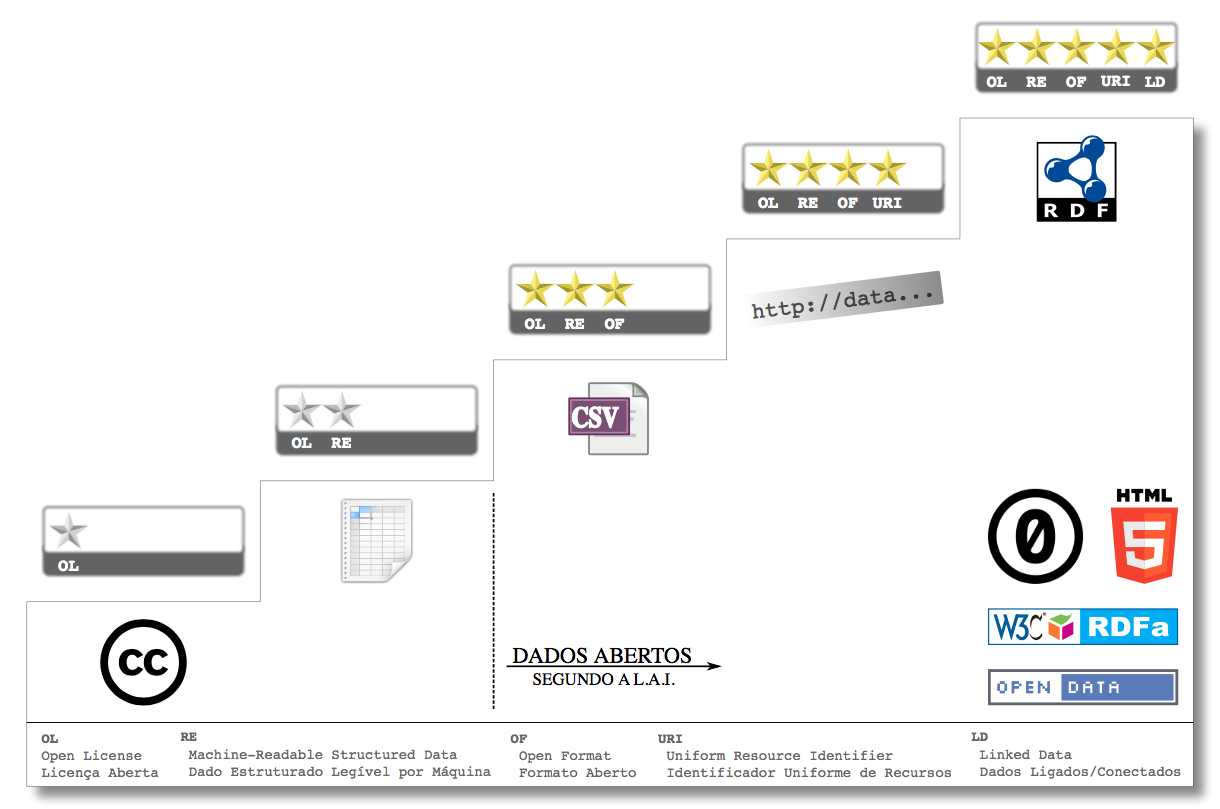
\includegraphics[width=1.0\textwidth]{imagens/open_data_stars.png}
  \caption{Classificação dos dados abertos segundo a escala de 5 estrelas de Berners-Lee}
  \label{fig:LABEL_FIG_OPEN_STARS}
\end{figure}

\begin{itemize}

\item \textbf{1 estrela}: Disponibilizar o dado na web (em qualquer formato) sob uma licença aberta.

\item \textbf{2 estrelas}: Tornar o dado estruturado (exemplo: uma planilha no Excel ao invés de uma imagem digitalizada de uma tabela).

\item \textbf{3 estrelas}: Tornar o dado disponível em um formato aberto, não-proprietário (exemplo: CSV ao invés de XLS, do Excel).

\item \textbf{4 estrelas}: Utilizar URIs para denotar os dados, para que as pessoas possam referenciá-los.

\item \textbf{5 estrelas}: Conectar os dados a outros datasets a fim de fornecer um contexto (\textit{linked data}\footnote{O conceito de linked data (dados ligados entre si) é um conjunto de práticas introduzidas por Tim Berners-Lee, com função de publicar e estruturar dados na Web, agregando valor semântico aos dados.}).

\end{itemize}



{\large Dados Abertos Governamentais}

Apesar de as definições de dados abertos serem gerais o suficiente para qualquer contexto, foram elaborados princípios mais específicos como referência para dados abertos governamentais, isto é, dados abertos sob posse de um governo\cite{REF_OGD_PRINCIPLES}. Um grupo de trabalho de 30 pessoas situado na Califórnia, Estados Unidos, o \textit{Open Government Working Group}, chegou a um consenso sobre os seguintes princípios:

\begin{enumerate}
\item \textbf{Completos}. Todos os dados públicos são disponibilizados. Dados são informações eletronicamente gravadas, incluindo, mas não se limitando a, documentos, bancos de dados, transcrições e gravações audiovisuais. Dados públicos são dados que não estão sujeitos a limitações válidas de privacidade, segurança ou controle de acesso, reguladas por estatutos.

\item \textbf{Primários}. Os dados são publicados na forma coletada na fonte, com a mais fina granularidade possível, e não de forma agregada ou transformada.

\item \textbf{Atuais}. Os dados são disponibilizados o quão rapidamente seja necessário para preservar o seu valor.

\item \textbf{Acessíveis}. Os dados são disponibilizados para o público mais amplo possível e para os propósitos mais variados possíveis.

\item \textbf{Processáveis por máquina}. Os dados são razoavelmente estruturados para possibilitar o seu processamento automatizado.

\item \textbf{Acesso não discriminatório}. Os dados estão disponíveis a todos, sem que seja necessária identificação ou registro.

\item \textbf{Formatos não proprietários}. Os dados estão disponíveis em um formato sobre o qual nenhum ente tenha controle exclusivo.

\item \textbf{Livres de licenças}. Os dados não estão sujeitos a regulações de direitos autorais, marcas, patentes ou segredo industrial. Restrições razoáveis de privacidade, segurança e controle de acesso podem ser permitidas na forma regulada por estatutos.
\end{enumerate}

Uma vez tendo em mãos esses dados, há diversos possíveis usos dos mesmos refletindo em diferentes aspectos da sociedade. Os DAGs trazem impacto direto na política e são causadores de um grande movimento de \textit{accountability}, isto é, uma responsabilidade aos governos a partir das informações oriundas desses dados. Dessa forma, podemos enxergar que quanto maior o acesso a essas informações, maiores as chances de que a sociedade acompanhe as iniciativas do poder público e as fiscalize, eventualmente contribuindo para a melhora do serviço público.

Outro grande reflexo dos DAGs é em termos de mercado. A partir da mineração dos dados abertos, que vêm como dados brutos, é possível extrair novas informações e agregá-las na forma de  produtos e serviços de valor para os usuários. Tem-se então a criação de novos negócios a partir dos DAGs. Alguns dos possíveis modelos de negócios a partir de DAGs e seus impactos na economia foram estudados por \cite{REF_MONO_BUUS}. 